\section{Question 4.1}

\subsection{Question}
\section{Introduction}
The \texttt{filevisitor.py} script, found in Listing \ref{listing:filevisitor}, was used to complete the bulk of the work in completing these exercises.  The scripts main function is to search the entire collection for documents and then perform a number of operations on each depending on its configuration.  It can be configured with specialized ``counter'' classes that process each document.  Two examples used are the \texttt{WordCounter} and \texttt{InlinkCounter} classes.  The \texttt{WordCounter} was used to determine word and bigram counts (Question 4.1), vocabulary size and growth (Question 4.2) and build an inverted index for the document collection (Question 5.8), while the \texttt{InlinkCounter}, you guessed it, built the in-link count (Question 4.8).

In addition to the \texttt{filevisitor.py} script two R scripts (\texttt{buildgraphs.R}, found in Listing \ref{listing:buildgraphs}, and \texttt{graphvocab.R}, found in Listing \ref{listing:graphvocab}), were used to create the graphics for each exercise.

Finally, to demonstrate the completed inverted index for exercise 5.8, the \texttt{search.py} script was created.  This script can be found in Listing \ref{listing:search}.

\section{Question 4.1}

\subsection{Question}
Plot rank-frequency curves (using a log-log graph) for words and bigrams in the Wikipedia collection available through the book website ( http://www.search-engines-book.com ). Plot a curve for the combination of the two. What are the best values for the parameter c for each curve?

\subsection{Approach}
The \texttt{FileVisitor} class recursed the directory structure, finding documents as it went.

\lstinputlisting[language=Python, caption={The FileVisitor Class}, label=listing:filevisitorclass,linerange={15-44},firstnumber=15]{code/filevisitor/filevisitor.py}

As it found files it performed various operations on them to complete the tasks required for the selected exercises.  This was done by calling the \texttt{counter.count} method, found on line 33, for each of the counters used on each file.  This count method and the recursive processing was very time consuming, so future work could improve upon this by parallelizing the task.

The BeautifulSoup library \cite{py:beautifulsoup} was used to remove the HTML tags, and then the NLTK library \cite{py:nltk} was used to tokenize the text.  Each word was then counted manually using the \texttt{count} method of the \texttt{WordCounter} class, found in Listing \ref{listing:wordcounter}, and the \texttt{bigram} method of the NLTK library \cite{py:nltk} was used to count the bigrams.  The \texttt{results} method then wrote these counts to a file which was used to create the resulting graphs.

\lstinputlisting[language=Python, caption={The WordCounter Class}, label=listing:wordcounter,linerange={46-97},firstnumber=46]{code/filevisitor/filevisitor.py}

\clearpage

\subsection{Results}
Output of running the \texttt{filevisitor.py} script can be found in Listing \ref{listing:filevisitorout}.

\lstinputlisting[language=bash, caption={filevisitor.py output}, label=listing:filevisitorout]{code/filevisitor/filevisitorout.txt}


The \texttt{buildgraph.R} script, found in Listing \ref{listing:buildgraphs}, was used to create the following graphs.  The word count graph can be found in Figure \ref{fig:wc}, the bigram count graph can be found in Figure \ref{fig:bigram}, and the graph showing the combination of the two can be found in Figure \ref{fig:both}.

\begin{figure}[h!]
\centering
\label{fig:wc}
\fbox{\includegraphics[scale=.55]{code/Rscripts/wc.pdf}}
\caption{Word Counts for Small Wikipedia Corpus}
\end{figure}

\begin{figure}[h!]
\centering
\label{fig:bigram}
\fbox{\includegraphics[scale=.55]{code/Rscripts/bg.pdf}}
\caption{Bigram Counts for Small Wikipedia Corpus}
\end{figure}

\begin{figure}[h!]
\centering
\label{fig:both}
\fbox{\includegraphics[scale=.55]{code/Rscripts/both.pdf}}
\caption{Both Word and Bigram Counts for Small Wikipedia Corpus}
\end{figure}


\subsection{Resources}
The textbook \textit{Search Engines: Information Retrieval in Practice} \cite{seirip}, the Python programming language \cite{python} with the python libraries Beautiful Soup \cite{py:beautifulsoup} and NLTK \cite{py:nltk}, and the R programming language \cite{rlang} were used to answer this question.

\subsection{Answer}
The wc.py script found in Listing \ref{listing:wordcount} was used to locate each file of the Wikipedia collection obtained from the book download page, available at \url{http://www.search-engines-book.com}.  The BeautifulSoup library was used to strip out the HTML tags and then the nltk library \cite{py:nltk} was used to tokenize the text.  The individual words were counted manually and the nltk library \cite{py:nltk} was used to count the bigrams.

The word count graph can be found in Figure \ref{fig:wc}, the bigram count graph can be found in Figure \ref{fig:bigram}, and the combination of the two can be found in Figure \ref{fig:both}.  The buildgraphs.R script was used to create these graphs and can be found in Listing \ref{listing:buildgraphs}.

\begin{figure}[h!]
\centering
\label{fig:wc}
\fbox{\includegraphics[scale=.55]{code/filevisitor/wc.pdf}}
\caption{Word Counts for Small Wikipedia Corpus}
\end{figure}

\begin{figure}[h!]
\centering
\label{fig:bigram}
\fbox{\includegraphics[scale=.55]{code/filevisitor/bg.pdf}}
\caption{Bigram Counts for Small Wikipedia Corpus}
\end{figure}

\begin{figure}[h!]
\centering
\label{fig:both}
\fbox{\includegraphics[scale=.55]{code/filevisitor/both.pdf}}
\caption{Both Word and Bigram Counts for Small Wikipedia Corpus}
\end{figure}
